\documentclass[10pt]{article}
\usepackage[utf8]{inputenc}
\usepackage[T1]{fontenc}
\usepackage{amsmath}
\usepackage{amsfonts}
\usepackage{amssymb}
\usepackage[version=4]{mhchem}
\usepackage{stmaryrd}
\usepackage{graphicx}
\usepackage[export]{adjustbox}
\graphicspath{ {./images/} }

\begin{document}
\section*{Math 141 Tutorial 8 Solutions}
\section*{Main problems}
\begin{enumerate}
  \item Consider the following problems on volumes of revolution using cylindrical shells.\\
(a) Find the volume of the object created by rotating the region trapped between $y=\ln \left(x^{2}\right)$, the $x$-axis, $x=1$ and $x=\sqrt{e}$ about the $y$-axis.\\
(b) Find the volume of the object created by rotating the region trapped between $y=x$ and $y=x^{2}$ about the line $y=1$
\end{enumerate}

\section*{Solution:}
(a) Notice that the area of the region trapped between $y=\ln \left(x^{2}\right)$, the $x$-axis, $x=1$ and $x=\sqrt{e}$ can be evaluated by integrating with respect to $x$. In doing so, one can imagine that we are "adding up" infinitely many vertical segments. Rotating one of these vertical segment at $x$ about the $y$-axis, we obtain a cylinder. The area of each cylinder is

$$
A(x)=2 \pi r(x) h(x)
$$

where the height is $h(x)=\ln \left(x^{2}\right)=2 \ln (x)$. Furthermore, since we are rotating about the $y$-axis the, radius of each cylinder will simply be the value of $x$. Put otherwise, $r(x)=x$. Hence

$$
A(x)=2 \pi x(2 \ln (x))=4 \pi x \ln (x)
$$

Since the object is obtained by "gluing together" these cylindrical shells, the volume is

$$
V=4 \pi \int_{1}^{\sqrt{e}} x \ln (x)
$$

To evaluate this integral, we integrate by parts with $u=\ln (x)$ and $\mathrm{d} v=x \mathrm{~d} x$. Hence, we have $\mathrm{d} u=\frac{1}{x} \mathrm{~d} x$ and we may pick $v=\frac{x^{2}}{2}$. Ergo,

$$
V=4 \pi\left(\left.\frac{1}{2} x^{2} \ln (x)\right|_{1} ^{\sqrt{e}}-\frac{1}{2} \int_{1}^{\sqrt{e}} x \mathrm{~d} x\right)=\pi\left[x^{2}(2 \ln (x)-1)\right]_{1}^{\sqrt{e}}=\pi
$$

(b) Since we wish to use the method of cylindrical shells, we will imagine horizontal segments that "add up" to the area of our region. We choose horizontal segments since, when rotated about the line $y=1$, these segments will form cylinders (vertical segments would form washers instead).\\
Thus, we notice that the area of the region trapped between $y=x$ and $y=x^{2}$ can be obtained by integrating with respect to $y$. Given a fixed $y \in[0,1]$, we can imagine the\\
horizontal segment from the curve $y=x$ to the curve $y=x^{2}$. Therefore, for this fixed $y$, the horizontal segment ranges from $x=y$ to $x=\sqrt{y}$. It follows that the length of this segment is $\sqrt{y}-y$. Now, rotating this segment about the line $y=1$ we obtain a cylinder. The area of this cylinder is

$$
A(y)=2 \pi r(y) h(y)
$$

where $r(y)$ is the radius and $h(y)$ is the height of the cylinder. The height is precisely the length of the segment that we rotated, or $h(y)=\sqrt{y}-y$. The radius of the cylinder is $1-y$ since we are rotating about the line $y=1$. Ergo

$$
A(y)=2 \pi(1-y)(\sqrt{y}-y)=2 \pi\left(y^{2}-y^{3 / 2}-y+y^{1 / 2}\right)
$$

We conclude that

$$
\begin{aligned}
V=\int_{0}^{1} A(y) \mathrm{d} y & =2 \pi \int_{0}^{1}\left(y^{2}-y^{3 / 2}-y+y^{1 / 2}\right) \mathrm{d} y \\
& =2 \pi\left[\frac{y^{3}}{3}-\frac{y^{5 / 2}}{5 / 2}-\frac{y^{2}}{2}+\frac{y^{3 / 2}}{3 / 2}\right]_{0}^{1}=\frac{\pi}{5}
\end{aligned}
$$

\begin{enumerate}
  \setcounter{enumi}{1}
  \item Using disks or cylindrical shells, find the volume of each object.\\
(a) The object created by rotating the region in the first quadrant trapped between $y=$ $x^{2} \sqrt{1-x}$ and $y=0$ about the line $x=-1$.\\
(b) The object created by rotating the region in the first quadrant trapped between $y=|x-2|$, $y=|x-2|+1, x=1$ and $x=3$ about the line $y=-3$.
\end{enumerate}

\section*{Solution:}
(a) As a first step, we study the region in the first quadrant trapped between $y=x^{2} \sqrt{1-x}$ and $y=0$. To this end, we begin by finding the points at which the curves $y=x^{2} \sqrt{1-x}$ and $y=0$ intersect. That is, we solve

$$
x^{2} \sqrt{1-x}=0
$$

and find that the only solutions are $x=0$ and $x=1$. Hence, these will be the bounds of our region. To find the area of said region, we can integrate $x^{2} \sqrt{1-x}$ with respect to $x$ from 0 to 1 . Here, we can imagine that we are gluing together vertical segment of height $x^{2} \sqrt{1-x}$ along the $x$ axis (from $x=0$ to $x=1$ ). For fixed $x$, rotating one of these segments about the line $x=-1$ yields a cylinder of height $h(x)=x^{2} \sqrt{1-x}$. Furthermore, since we are rotating about $x=-1$, notice that the radius of said cylinder is $r(x)=x+1$. Thus, the cylinder has area

$$
A(x)=2 \pi r(x) h(h)=2 \pi(x+1) x^{2} \sqrt{1-x}
$$

It follows that the volume of the object is

$$
\begin{aligned}
V=\int_{0}^{1} A(x) \mathrm{d} x & =2 \pi \int_{0}^{1}(x+1) x^{2} \sqrt{1-x} \mathrm{~d} x \\
& =2 \pi \int_{0}^{1}(2-u)(1-u)^{2} \sqrt{u} \mathrm{~d} u \\
& =2 \pi \int_{0}^{1}\left(2 u^{1 / 2}-5 u^{3 / 2}+4 u^{5 / 2}-u^{7 / 2}\right) \mathrm{d} u \\
& =2 \pi\left[\frac{4}{3} u^{3 / 2}-2 u^{5 / 2}+\frac{8}{7} u^{7 / 2}-\frac{2}{9} u^{9 / 2}\right]_{0}^{1} \\
& =\frac{32}{63} \pi
\end{aligned}
$$

(b) Recall that

$$
|x|= \begin{cases}x & \text { if } x \geq 0 \\ -x & \text { if } x<0\end{cases}
$$

Hence,

$$
|x-2|= \begin{cases}x-2 & \text { if } x \geq 2 \\ 2-x & \text { if } x<2\end{cases}
$$

In particular, we will split our problem into two parts. The solid of revolution in question, whose volume we will denote $V$, is composed of two objects:

\begin{itemize}
  \item The object created by rotating the region trapped between $y=|x-2|, y=|x-2|+1$ , $x=1$ and $x=2$ about the line $y=-3$. We will call the volume of this object $V_{1}$
  \item The object created by rotating the region trapped between $y=|x-2|, y=|x-2|+1$ , $x=2$ and $x=3$ about the line $y=-3$. We will call the volume of this object $V_{2}$.\\
We begin by finding $V_{1}$. For $x \in[1,2]$, we can imagine de line segment from $y=|x-2|=$ $2-x$ to $y=|x-2|+2=2-x+1=3-x$. Rotating this segment about $y=-3$ we obtain a washer whose area is
\end{itemize}

$$
\begin{aligned}
A(x)=\pi(R(x))^{2}-\pi(r(x))^{2} & =\pi\left((R(x))^{2}-(r(x))^{2}\right) \\
& =\pi\left((3-x)^{2}-(2-x)^{2}\right) \\
& =\pi(5-2 x) .
\end{aligned}
$$

This washer corresponds to the cross sections our object. Hence,

$$
V_{1}=\int_{1}^{2} A(x) \mathrm{d} x=\pi \int_{1}^{2}(5-2 x) \mathrm{d} x=2 \pi
$$

Similarly (or by noting symmetry), we find that $V_{2}=2 \pi$. In conclusion, the volume is $V=V_{1}+V_{2}=4 \pi$.\\
3. The integral below represents the volume of a solid object obtained by rotating a region $R$ about the $x$-axis.

$$
\int_{0}^{\sqrt{\pi}} \pi \sin ^{2}\left(x^{2}\right) d x
$$

Find the volume obtained by rotating $R$ about the $y$-axis. Include a sketch of $R$ and the new solid in your solution.

\section*{Solution:}
If $R$ is a region such that the volume, after rotating about the $x$-axis is given by

$$
\int_{0}^{\sqrt{\pi}} \pi \sin ^{2}\left(x^{2}\right) d x
$$

then we can assume that the method of disks/washers was used. Hence, the cross sections of the solid of revolution obtained by rotating $R$ about the $x$-axis are disks of area

$$
\pi(r(x))^{2}=\pi \sin ^{2}\left(x^{2}\right)
$$

It follows that the radius of the disk is $\sin \left(x^{2}\right)$. We deduce that $R$ is the region between the curve $\sin \left(x^{2}\right)$ and the $x$-axis, with $x \in[0, \sqrt{\pi}]$ (as depicted below).\\
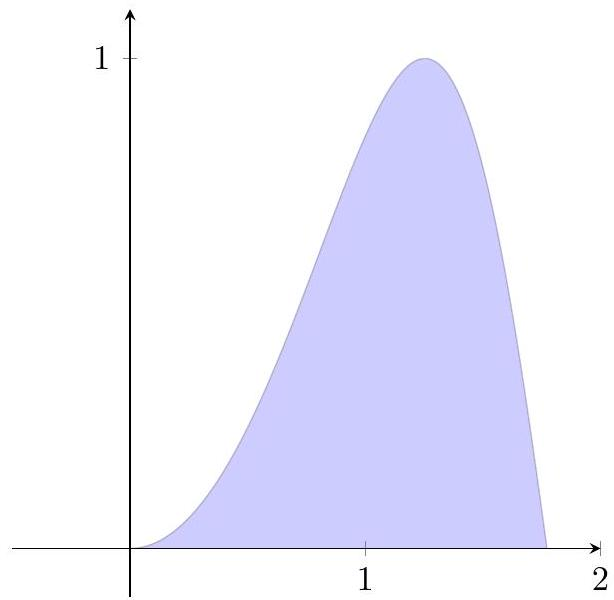
\includegraphics[max width=\textwidth, center]{2024_12_27_071a2f78100f58bfb468g-05}

Rotating $R$ about the $y$-axis we obtain a new solid. For fixed $x$, consider the segment from $y=0$ to $y=\sin \left(x^{2}\right)$. Rotating this segment about the $y$-axis yields a cylinder whose area is

$$
A(x)=2 \pi r(x) h(x)=2 \pi x \sin \left(x^{2}\right)
$$

Therefore, the volume obtained by rotating $R$ about the $y$-axis is

$$
V=2 \pi \int_{0}^{\sqrt{\pi}} x \sin \left(x^{2}\right) \mathrm{d} x \stackrel{u \mapsto x^{2}}{=} \pi \int_{0}^{\pi} \sin (u) \mathrm{d} u=-\left.\pi \cos (u)\right|_{0} ^{\pi}=2 \pi
$$

\begin{enumerate}
  \setcounter{enumi}{3}
  \item Find an interval $[a, b]$ of length 6 such that the average value of $x^{2}$ over $[a, b]$ is 4 .
\end{enumerate}

\section*{Solution:}
Recall that the average value of the function $f(x)=x^{2}$ over any interval $[a, b]$ is defined to be the integral

$$
\frac{1}{b-a} \int_{a}^{b} x^{2} \mathrm{~d} x
$$

which, by the Fundamental Theorem of Calculus, is precisely the expression

$$
\begin{aligned}
\frac{1}{b-a} \int_{a}^{b} x^{2} \mathrm{~d} x & =\frac{1}{b-a}\left(\left.\frac{x^{3}}{3}\right|_{x=a} ^{x=b}\right) \\
& =\frac{b^{3}-a^{3}}{3(b-a)} \\
& =\frac{(b-a)\left(b^{2}+a b+a^{2}\right)}{3(b-a)} \\
& =\frac{b^{2}+a b+a^{2}}{3} .
\end{aligned}
$$

Hence, the average value of $x^{2}$ over an interval $[a, b]$ is 4 if and only if

$$
\frac{b^{2}+a b+a^{2}}{3}=4
$$

or, equivalently,

$$
b^{2}+a b+a^{2}=12
$$

Using also that the length of the interval is 6 , we know that $b-a=6$. Substituting $b=a+6$ in our last equation we obtain

$$
(a+6)^{2}+a(a+6)+a^{2}=12
$$

or, equivalently

$$
a^{2}+6 a+8=(a+4)(a+2)=0
$$

Hence, we find that the possible values for $a$ are -4 and -2 .\\
We find two solutions: the intervals $[-4,2]$ and $[-2,4]$ are of length 6 and such that $x^{2}$ has an average value of 4 on these intervals.\\
5. Determine whether each improper integral is convergent or divergent and justify your statement. When convergent, is it always possible to compute the value of the improper integral? If so, compute it.\\
(a) $\int_{1}^{2} \frac{1}{(x-2)^{2}} \mathrm{~d} x$\\
(b) $\int_{0}^{\infty} \sin \theta e^{\cos \theta} \mathrm{d} \theta$\\
(c) $\int_{0}^{10} \frac{1}{x^{2}+6 x-55} \mathrm{~d} x$

\section*{Solution:}
(a) Here, the integrand $\frac{1}{(x-2)^{2}}$ is continuous everywhere except at $x=2$. Therefore, this is an improper integral. To determine whether or not it converges, we need to investigate the limit

$$
\begin{aligned}
\lim _{t \rightarrow 2^{-}} \int_{1}^{t} \frac{1}{(x-2)^{2}} \mathrm{~d} x & =\lim _{t \rightarrow 2^{-}}\left(-\left.\frac{1}{(x-2)}\right|_{x=1} ^{x=t}\right) \\
& =-\lim _{t \rightarrow 2^{-}}\left(\frac{1}{t-2}+1\right)
\end{aligned}
$$

which does not converge because the limit

$$
\lim _{t \rightarrow 2^{-}} \frac{1}{t-2}=-\infty
$$

is divergent. Hence, the given improper integral is divergent.\\
(b) Since we are integrating on the unbounded interval $[0, \infty)$, this is an improper integral. To determine whether or not it is convergent, we investigate the following limit:

$$
\lim _{t \rightarrow \infty} \int_{0}^{t} \sin \theta e^{\cos \theta} \mathrm{d} \theta
$$

By making the $u$-substitution $u=\cos (\theta)$ (giving $\mathrm{d} u=-\sin (\theta)$ ), we can find an antiderivative for $\sin (\theta) e^{\cos (\theta)}$ :

$$
\int \sin \theta e^{\cos \theta} \mathrm{d} \theta=\int-e^{u} \mathrm{~d} u=-e^{u}+C=-e^{\cos (\theta)}+C
$$

where $C$ is an arbitrary constant. Using this antiderivative, we can evaluate $\int_{0}^{t} \sin \theta e^{\cos \theta} \mathrm{d} \theta$ for any $t>0$ :

$$
\begin{aligned}
\int_{0}^{t} \sin \theta e^{\cos \theta} \mathrm{d} \theta & =\left(-\left.e^{\cos \theta}\right|_{\theta=0} ^{\theta=t}\right) \\
& =1-e^{\cos t}
\end{aligned}
$$

Thus,

$$
\lim _{t \rightarrow \infty} \int_{0}^{t} \sin \theta e^{\cos \theta} \mathrm{d} \theta=\lim _{t \rightarrow \infty}\left(1-e^{\cos t}\right)
$$

Since $\lim _{t \rightarrow \infty} e^{\cos (t)}$ is divergent, we infer that the improper integral

$$
\int_{0}^{\infty} \sin \theta e^{\cos \theta} \mathrm{d} \theta
$$

is divergent as well.\\
(c) To check whether this is an improper integral, we check for discontinuities of the integrand in the interval $[0,10]$. This is easiest when we factor the denominator of our rational function:

$$
\frac{1}{x^{2}+6 x-55}=\frac{1}{(x+11)(x-5)}
$$

Clearly, the denominator is zero when $x=5$ (which is a point in the interval $[0,10]$ over which we are integrating). Therefore, this is an improper integral. Now, because the discontinuity point is not an endpoint of the interval on which we are integrating, we must split our integral into two improper integrals of the second type:

$$
\int_{0}^{10} \frac{1}{(x+11)(x-5)} \mathrm{d} x=\int_{0}^{5} \frac{1}{(x+11)(x-5)} \mathrm{d} x+\int_{5}^{10} \frac{1}{(x+11)(x-5)} \mathrm{d} x .
$$

To evaluate each of these, we first need a partial fraction decomposition for: $\frac{1}{(x+11)(x-5)}$. That is, we seek constants $A, B$ such that

$$
\frac{1}{(x+11)(x-5)}=\frac{A}{x+11}+\frac{B}{x-5}
$$

Multiplying both sides by $(x+11)(x-5)$ yields the equation

$$
1=A(x-5)+B(x+11)=(A+B) x+(11 B-5 A)
$$

Hence, $A+B=0$ and $11 B-5 A=1$. The first equation tells us that $B=-A$ so that

$$
1=11 B-5 A=16 B
$$

Thus, we have

$$
B=\frac{1}{16} \quad \text { and } \quad A=-\frac{1}{16}
$$

so that

$$
\frac{1}{(x+11)(x-5)}=\frac{1}{16(x-5)}-\frac{1}{16(x+11)}
$$

Returning to out integrals, we can evaluate

$$
\begin{aligned}
\int_{0}^{5} \frac{1}{(x+11)(x-5)} \mathrm{d} x & =\lim _{t \rightarrow 5^{-}} \int_{0}^{t}\left(\frac{1}{16(x-5)}-\frac{1}{16(x+11)}\right) \mathrm{d} x \\
& =\lim _{t \rightarrow 5^{-}}\left[\frac{1}{16} \ln |x-5|-\frac{1}{16} \ln |x+11|\right]_{0}^{t} \\
& =\lim _{t \rightarrow 5^{-}} \frac{1}{16}[\ln (5-t)-\ln (5)-\ln (t+11)+\ln (11)] \\
& =\frac{1}{16}\left[\lim _{t \rightarrow 5^{-}} \ln (5-t)-\ln (5)-\ln (16)+\ln (11)\right]
\end{aligned}
$$

\section*{Page 8}
Since $\lim _{t \rightarrow 5^{-}} \ln (5-t)$ does not exist, the integral $\int_{0}^{5} \frac{1}{(x+11)(x-5)} \mathrm{d} x$ is divergent. It follows that

$$
\int_{0}^{10} \frac{1}{(x+11)(x-5)} \mathrm{d} x
$$

also diverges.

Page 9

\section*{Extra Practice problems:}
\begin{enumerate}
  \item Consider the object created by rotating the region trapped between $y=x$ and $y=x^{2}$ about the $y$-axis.\\
(a) Find the volume using disks.\\
(b) Find the volume using cylindrical shells.
  \item Find the volume of the object created by rotating the region in the first quadrant trapped between $f(x)=|x|, y=1-|x|$ and $x=0$ about the $y$-axis.
  \item Find the volume of the object created by rotating the region in the first quadrant trapped between $y=x$ and $y=\sqrt{x}$ about the $x$-axis.
  \item Find the volume of the object created by rotating the region bounded by the curves $x=0$ and $x=9-y^{2}$ about $x=-1$.
  \item Find the volume of the object created by rotating the region bounded by the curves $y=x^{2}+1$ and $y=9-x^{2}$ about $y=-1$.
  \item A bathtub which can hold a maximum of 300 litres is currently filled with 290 liters of water. At time $t=0$, water begins to pour into the tub at a (varying) rate of $10 \sqrt{t}$ litres per minute, while at the same time water begins to drain out of the tub at a rate of $2 t^{2}$ litres per minute (where $t$ is measured in minutes). Assuming these rates continue indefinitely, does the bathtub overflow?
  \item Compute the average value of the function $f(x)=\frac{e^{1 / x}}{x^{2}}$ on $[1,4]$.
\end{enumerate}

\end{document}